%Copyright 2014 Jean-Philippe Eisenbarth
%This program is free software: you can 
%redistribute it and/or modify it under the terms of the GNU General Public 
%License as published by the Free Software Foundation, either version 3 of the 
%License, or (at your option) any later version.
%This program is distributed in the hope that it will be useful,but WITHOUT ANY 
%WARRANTY; without even the implied warranty of MERCHANTABILITY or FITNESS FOR A 
%PARTICULAR PURPOSE. See the GNU General Public License for more details.
%You should have received a copy of the GNU General Public License along with 
%this program.  If not, see <http://www.gnu.org/licenses/>.

%Based on the code of Yiannis Lazarides
%http://tex.stackexchange.com/questions/42602/software-requirements-specification-with-latex
%http://tex.stackexchange.com/users/963/yiannis-lazarides
%Also based on the template of Karl E. Wiegers
%http://www.se.rit.edu/~emad/teaching/slides/srs_template_sep14.pdf
%http://karlwiegers.com
\documentclass{scrreprt}
\usepackage{listings}
\usepackage{underscore}
\usepackage[bookmarks=true]{hyperref}
\usepackage[utf8]{inputenc}
\usepackage[english]{babel}
\usepackage{pgfgantt}
\usepackage{CJKutf8}
\usepackage{graphicx}
\hypersetup{
    bookmarks=false,    % show bookmarks bar?
    pdftitle={Software Requirement Specification},    % title
    pdfauthor={Jean-Philippe Eisenbarth},                     % author
    pdfsubject={TeX and LaTeX},                        % subject of the document
    pdfkeywords={TeX, LaTeX, graphics, images}, % list of keywords
    colorlinks=true,       % false: boxed links; true: colored links
    linkcolor=blue,       % color of internal links
    citecolor=black,       % color of links to bibliography
    filecolor=black,        % color of file links
    urlcolor=purple,        % color of external links
    linktoc=page            % only page is linked
}%
\def\myversion{1.0 }
\date{}
%\title
\usepackage{hyperref}
\begin{document}

\begin{flushright}
    \rule{16cm}{5pt}\vskip1cm
    \begin{bfseries}
        \Huge{SOFTWARE REQUIREMENTS\\ SPECIFICATION}\\
        \vspace{1.9cm}
        for\\
        \vspace{1.0cm}
        $<$chatroom robot assistant$>$\\
        \vspace{1.0cm}
        \LARGE{Version \myversion approved}\\
        \vspace{1.0cm}
	\begin{CJK}{UTF8}{bkai}
        		 Prepared by :  \\
	   	1031408 劉彥呈\\
	   	1031452 何浩璘\\
	   	1033329 林仕翔\\
	   	1033336 尹法堯\\
        		1041459 梁澤洲\\
        \vspace{1.0cm}
        $<$開放平台軟體 第15組$>$\\
        \vspace{1.0cm}
        \today\\
	\end{CJK}
    \end{bfseries}
\end{flushright}

\tableofcontents


\chapter*{Revision History}

\begin{CJK}{UTF8}{bkai}
	\begin{center}
    		\begin{tabular}{|c|c|c|c|c|}
        		\hline
	    	學號 & Name & Date & Reason For Changes & Version\\
        		\hline
	   	1031408 & 劉彥呈 & 5/19 & 顯示時間 & 1\\
        		\hline
	    	1033336 & 尹法堯 & 5/19 & Client進入訊息 & 2\\
        		\hline
		1031408 & 劉彥呈 & 5/20 & Client離開訊息 & 3\\
        		\hline
		1033336 & 尹法堯 & 5/20 & 區分相同的name & 4\\
        		\hline
		1033336 & 尹法堯 & 6/14 & 完成資料庫所有功能和Server新增帳號 & 5\\
		\hline
		1031408 & 劉彥呈 & 6/14 & 完成資料庫與介面的互動 & 5\\
        		\hline
		1031408 & 劉彥呈 & 6/17 & 顯示再現人數 & 7\\
        		\hline
		1033336 & 尹法堯 & 6/18 &  Server刪除帳號& 8\\
        		\hline
		1031408 & 劉彥呈 & 6/19 & Server踢除Client & 9\\
        		\hline
		1031452 & 何浩璘 & 6/19 & Bot加入以及weather-api的使用 & 10\\
        		\hline
		1031408 & 劉彥呈 & 6/19 & 更換介面的顏色 & 11\\
        		\hline
		1031452 & 何浩璘 & 6/23 & Bot增加匯率轉換-api和顯示日期區域時間 & 12\\
        		\hline
    		\end{tabular}
	\end{center}


\chapter{Introduction}

\section{Purpose}
該文件提供cahtroom robot assistant Version12的相關說明,包含改產品的開發理念、最終
成果,產品的提供對象及適用範圍,系統的程式碼架構,不同物件之間的上下關係,程式運行環境以及產品特色

\section{Document Conventions}
$<$Describe any standards or typographical conventions that were followed when 
writing this SRS, such as fonts or highlighting that have special significance.  
For example, state whether priorities  for higher-level requirements are assumed 
to be inherited by detailed requirements, or whether every requirement statement 
is to have its own priority.$>$

\section{Intended Audience and Reading Suggestions}
本文件適合以下職位的人員觀看,部分內容須有程式邏輯相關知識: \\
(1)專案經理:專案經理可以根據該文檔瞭解預期產品的功能,以此進行系統設計。 \\
(2)設計員:對需求進行分析,並設計出系統,包括資料庫的設計。 \\
(3)程式師:瞭解系統功能,對後續更新版本或產品維護提供程式架構。 \\
(4)測試員:根據本文檔對軟體產品進行功能性測試和非功能性測試。 \\
(5)銷售人員:瞭解預期產品的功能和性能。 \\
(6)用戶:瞭解預期產品的功能和性能,與分析人員對整個需求進行討論和協商。 \\


\section{Project Scope}
該產品的開發理念為節省使用者在聊天室與夥伴聊天時,為查詢生活中的小資訊而必須頻繁切換應用程式的時間
,希望使用者可以在與夥伴聊天時,在時間上有很好的使用者體驗,或者討論單日行的旅遊,或者與分隔兩地的朋友聊天時,
可以方便的查詢當地天氣相關資訊以提供聊天話題。

\section{References}
1. https://pypi.org/project/weather-api/ \\
2. https://pypi.org/project/currency.converter/ \\
3. http://pyqt.sourceforge.net/Docs/PyQt5/ \\
4.https://github.com/mongodb/mongo-python-driver\\
5.https://pip.pypa.io/en/stable/\\




\chapter{Overall Description}

\section{Product Perspective}
\begin{figure}[ht]
\begin{center}
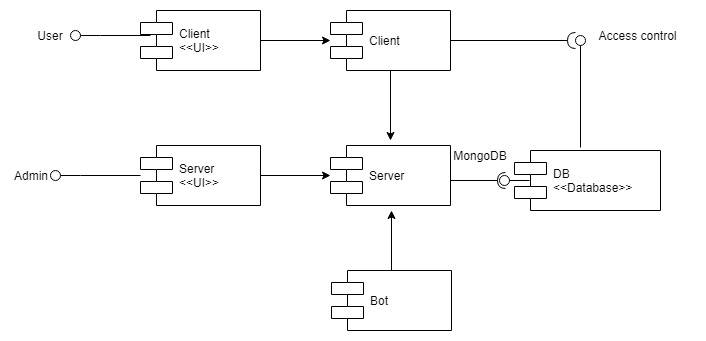
\includegraphics[width=17cm]{Component.jpg}
\end{center}
\caption{Component}
\label{fig:1}
\end{figure}

\newpage
\section{Product Functions}
\begin{figure}[ht]
\begin{center}
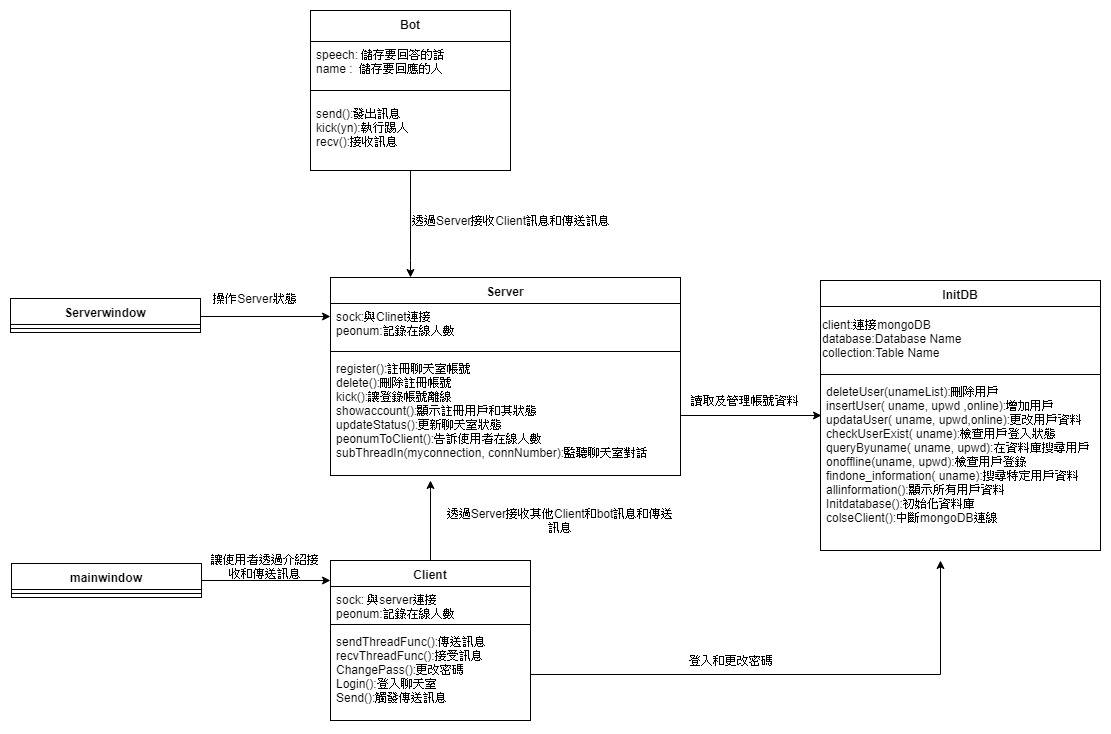
\includegraphics[width=17cm]{Class.jpg}
+\end{center}
\caption{Class}
\label{fig:1}
\end{figure}

\section{User Classes and Characteristics}
$<$Identify the various user classes that you anticipate will use this product.  
User classes may be differentiated based on frequency of use, subset of product 
functions used, technical expertise, security or privilege levels, educational 
level, or experience. Describe the pertinent characteristics of each user class.  
Certain requirements may pertain only to certain user classes. Distinguish the 
most important user classes for this product from those who are less important 
to satisfy.$>$

\section{Operating Environment}
1. OS: Window7 以上版本 (未在其他作業系統測試過) \\
2. 開發語言: python3 \\
3. 使用python api: weather-api, currency_converter \\
4. 其他python開發套件: socket, threading, os, sys, time, PyQt5 \\
5. 資料庫: mongoDB

\section{Design and Implementation Constraints}
本產品由自由團隊開發,不存在可能限制產品的開發項目之公司相關規定,亦不涉及法律相關的問題。本產品所使用的資料庫為mongoDB,開發者需要擁有基礎的資料庫知識,以及mongoDB相關的語法,開發語言為python3,開發者可能需要python3開發之經驗。

\section{User Documentation}
本產品目前唯一的文件為本文件,亦無額外的操作手冊。

\section{Assumptions and Dependencies}

本產品使用了mongoDB與python3支援的額外之函示庫,未來如果函示庫在使用之方法上有重大之改變將會嚴重影響該產品之功能,該產品使用的額外函示庫請參照文件內文之3.2部分。





\chapter{External Interface Requirements}

\section{User Interfaces}
\begin{figure}[h]
\begin{center}
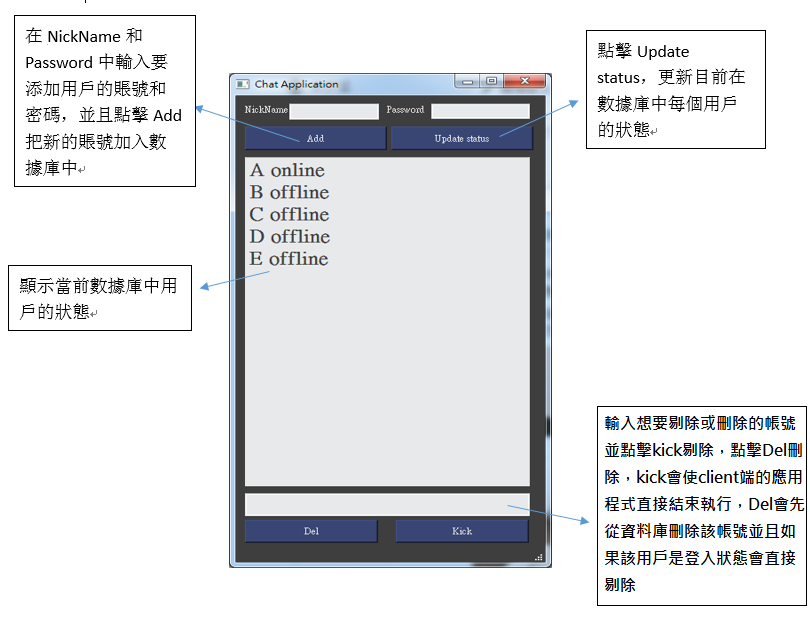
\includegraphics[width=15cm]{interface1.png}
+\end{center}
\caption{sever interface}
\label{fig:2}
\end{figure}

\begin{figure}[h]
\begin{center}
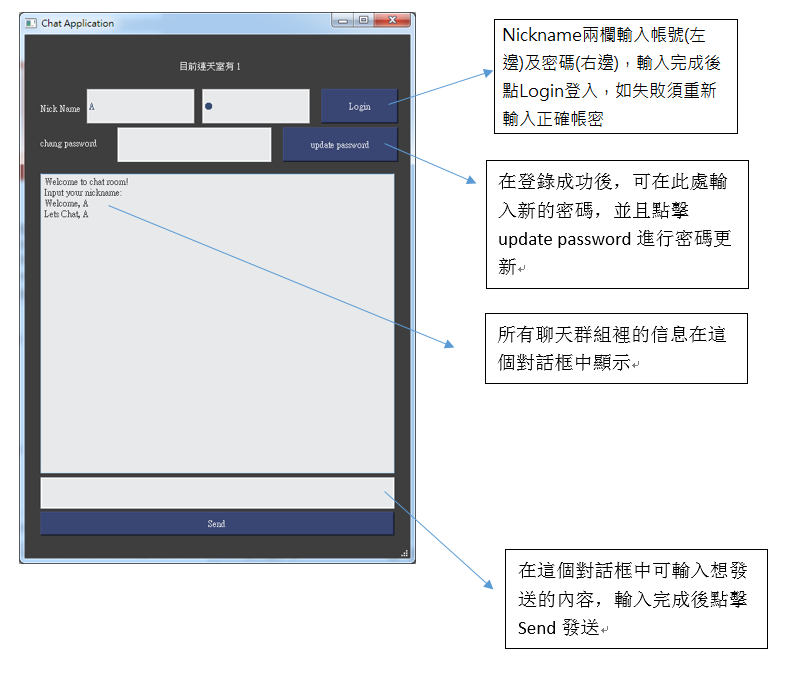
\includegraphics[width=15cm]{interface2.png}
\end{center}
\caption{client interface}
\label{fig:3}
\end{figure}



\section{Software Interfaces}
一、 資料庫 \\
(1) mongoDB 3.6 : 用於管理帳號密碼以及狀態資訊 \\
二、python 套件 \\
(1) socket : 用於處理server與client之間的訊息傳遞 \\
(2) threading : 用與處理接收訊息、傳遞訊息、GUI之間的線程管理 \\
(3) os : 用於強制讓程式結束運作\\
(4) time : 用於顯示發送或接收訊息時,當下的時間資訊\\
(5) PyQt5 5.10.1 : 用於呈現server與client的UI介面、按鈕事件控制\\
(6) pymongo 3.6.4 : python用於控制mongoDB的函示庫\\
(7) weather-api 1.0.4 : 用於取得某地的天氣資訊,輸入為地區名稱,輸出會當地溫度、天氣狀況、濕度等資訊\\
(8) CurrencyConverter 0.13.5 : 用於轉換兩個不同的貨幣,輸入為金額、原始貨幣、轉換後貨幣,輸出為轉換後貨幣的金額 \\

\section{Communications Interfaces}
本產品要求使用者要有正常的網路環境,來處理與伺服器之間的連線,伺服器亦不可將用於接收傳送的port使用防火牆擋住,須開放來自外來的連線需求。


\chapter{System Features}


\section{Fast Search Weather and Exchange rate Information}
該特色可以幫助使用者快速的取得特定地區的天氣資訊以及兩個不同貨幣之間的貨幣量值轉換

\subsection{Description and Priority}
基於希望使用者可以直接在聊天室取得簡單的資訊並節省時間的目的,我們初步完成了能查詢天氣資訊和匯率轉換的功能。這兩項功能的好處是,假如三五好友利用閒暇的時間在討論想去哪裡玩時,可以直接向連天室的機器人詢問當地氣候,可以讓連天室的討論快速的進行下去,又或者與分隔兩地的人交談時,可以快速的查詢對方當地的氣候,順利的找到話題並繼續聊天。匯率的部分可以在討論該去哪個國家玩時,或者已經決定要去哪個國家時,可以方便的查詢目前的匯率決定換錢的時機,這兩個特色可以簡單的就在聊天室向機器人詢問取得,而不需要再切換額外的應用程式查詢。

\subsection{Stimulus/Response Sequences}
以下舉例使用者實際上需要輸入的句子以及得到的答案: \\
(1) 使用者輸入 - bot weather 桃園 	機器人回復 - Taoyuan City Mostly Clear 27\\
表示桃園目前的天氣晴朗,並且溫度是27度\\
(2) 使用者輸入 - bot convert 1000 JPY USD 		機器人回復 - 1000 JPY=9.065600246097056 USD\\
使用首先輸入bot convert,接著輸入須轉換金額,接著輸入轉換的原始貨幣再輸入轉換後貨幣,以上面的例子,我們可以得到1000日幣約等於9美元\\

\subsection{Functional Requirements}
(1) 詢問氣候 : 使用者登入後在client端的UI上輸入 --- bot weather 桃園 --- 指令,bot幫助程式判斷我現在要詢問的對象是機器人,接著weather代表要詢問的事情是天氣的資訊,地點是桃園,server收到訊息後,從指令中取得weather-api所需的字句,取得答案後將答案送給client,client進而把取得的資訊顯示在UI上\\
(2) 詢問匯率轉換 : 使用者在client端的UI輸入 ---  bot convert 1000 JPY USD --- 指令,bot幫助程式判斷我現在要詢問的對象是機器人,接著convert代表要詢問的是貨幣的轉換,需要轉換的金額是1000,原始貨幣是日圓,轉換後貨幣是美元,server收到訊息後,從指令中取得CurrencyConverter所需的字句,取得答案後將答案送給client,client進而把取得的資訊顯示在UI上\\



\chapter{Other Nonfunctional Requirements}


\section{Safety Requirements}
Client在發送訊息時,會有兩個指令會造成錯誤:\\
(1)systeM==!!:是使用者登入時,告訴Server現在有一個用戶要登入了,並統計人數,告訴所有的Client現在的在線人數是多少。\\
(2)kick==:它是Server會發送訊息告訴Client,經由Client辨別,來決定是否主動斷開連線。\\
在Server介面時,當有兩個以上使用者在登入時,要等待所有使用者登入完畢,不能有一位登入,其他還未登入時,使用Kick功能,這會造成Server的損壞。\\


\section{Security Requirements}
目前只有針對帳號密碼登入時,把它們與資料庫進行比對,比對錯誤將會有訊息顯示在client端的UI要求重輸,沒有其他包含針對資料庫或連線進行惡意攻擊的防護措施

\section{Software Quality Attributes}

該產品擁有高度的可測試性及可維護性: \\
(1)可測試性: 該產品在開發中皆可使用簡易的輸出行為來測試結果,測試員可使用單個裝置扮演server以及多個client的角色,進行交互測試。\\
(2)可維護性: 該產品開發中所使用的程式變數皆為有意義之命名,function之間功能的獨立性亦非常明確,功能修改以及新增皆非常容易。\\

\section{Business Rules}
此產品關於client端存在類似管理員的角色,只要client知道特殊的密碼,便可以使用該密碼進行剔除連天室其他用戶的動作,輸入指令為 - bot kick (nickname) - ,輸入後系統會要求輸入特殊的密碼,輸入正確即可踢除用戶,被剔除的用戶將會被強制斷線並關閉應用程式。


\chapter{Other Requirements}
$<$Define any other requirements not covered elsewhere in the SRS. This might 
include database requirements, internationalization requirements, legal 
requirements, reuse objectives for the project, and so on. Add any new sections 
that are pertinent to the project.$>$

\section{Appendix A: Glossary}
%see https://en.wikibooks.org/wiki/LaTeX/Glossary
$<$Define all the terms necessary to properly interpret the SRS, including 
acronyms and abbreviations. You may wish to build a separate glossary that spans 
multiple projects or the entire organization, and just include terms specific to 
a single project in each SRS.$>$


\section{Appendix C: To Be Determined List}
$<$Collect a numbered list of the TBD (to be determined) references that remain 
in the SRS so they can be tracked to closure.$>$

\end{CJK}
\end{document}
